\chapter{Manual de Usuario}
\title{Manual de Usuario}
\label{cap:ManualDeUsuario}

A continuación se detalla un pequeño manual de usuario para aquellos astrónomos ya sean  \textit{amateurs} o profesionales. También se establece para aquellas personas que tengan la curiosidad de descubrir el mundo de la astronomía a través de este prototipo de cliente web basado en INDI.

\section{Previo}
Antes de comenzar diremos, que si se va a iniciar el prototipo desde un ordenador y se desea lanzar un simulador hay que realizar los siguientes pasos:
\begin{itemize}
  \item Instalar INDI. Para ello hay que instalar INDI en la máquina como dicen los pasos del propio tutorial de la página\cite{InstalarINDI}
  \item Lanzar Simulador INDI\ref{fig:INDIServer}. Para lanzar un simulador INDI hay que abrir un terminal en Linux\cite{Linux} y escribir la siguiente instrucción si se desea lanzar por ejemplo un telescopio: \textit{indiserver indi\_simulator\_telescope}
\end{itemize}

Al presionar la tecla Enter, hemos lanzado nuestro simulador de telescopio, en este caso. Si se desea lanzar otro simulador tiene que proceder de la misma manera, o sea, repetir la operación de la forma “Lanzar Simulador INDI” y cambiar el nombre del dispositivo por el que se desea ejecutar. Por ejemplo: \textit{indiserver indi\_simulator\_ccd} o \textit{indiserver indi\_simulator\_gps}.\\

La lista de dispositivos se puede consultar en la dirección que a continuación se facilita.\cite{ListaDispositivos}

\begin{figure}[htb]
\centering
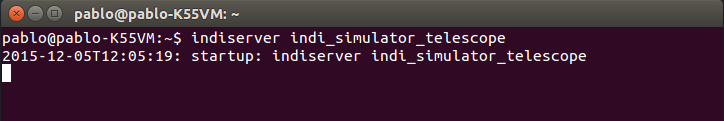
\includegraphics[width=1\textwidth]{./imagenes/capturaINDIServer}
\caption{Lanzamiento del Simulador de Telescopio} \label{fig:INDIServer}
\end{figure}

\section{Lanzando el Prototipo de Cliente}
Una vez que está lanzado el simulador con el que vamos a trabajar, tenemos que abrir el fichero principal denominado \textit{parser.html}.

En el momento que tengamos abierto el fichero \textit{parser.html} en el navegador, se nos solicitará una IP y un puerto válido que corresponderá con un servidor INDI.
